\section{The Initial Plan}
	\subsection{Overview}
		The initial plan was to determine an adequate RISC-V softcore for the mixed hardware and software modifications that were intended to be completed. The chosen core was RPU. Once selected, this core was to be uploaded onto an FPGA, and brought to an operational level with an OS running on it. At this stage, a series of test algorithms would be run with metrics collected in order to establish a baseline of performance. This baseline was to be used to contrast against the improved softcore implementations. First, several dark silicon methodologies were to be implemented individually, then successful methodologies were to be merged into a final working model. This final working model would be used to produce the data for the final A visual outline of this is shown in Figure~\ref{ThesisFlowchart}. 
		
		\begin{figure}
			\centering
			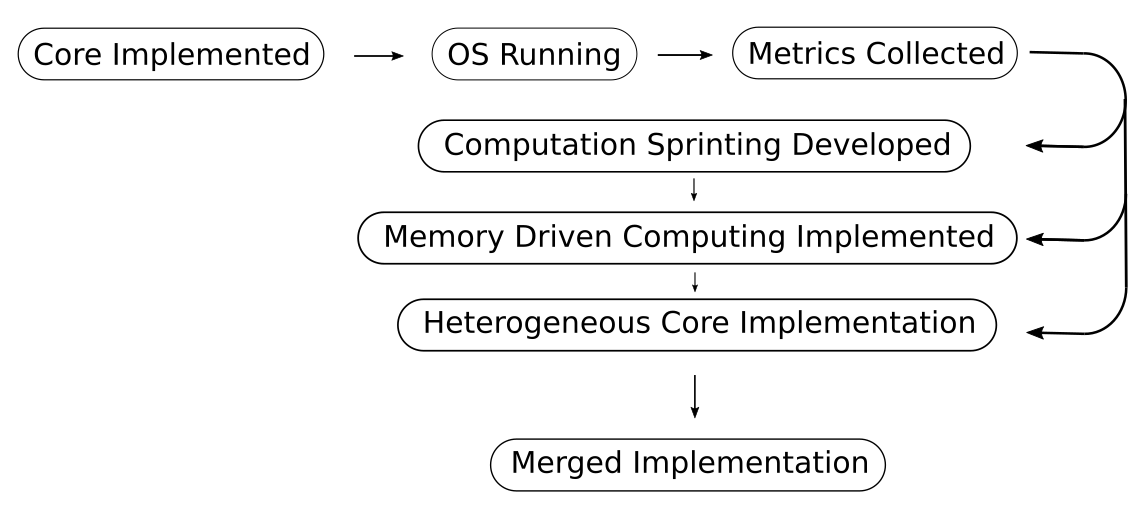
\includegraphics[width=0.8\textwidth]{ThesisMethodFlowchart.png}
			\caption{Flowchart of Thesis implementation}
			\label{ThesisFlowchart}
		\end{figure}

	
	\subsection{Software Packages Used}
		\textbf{VMWare} - Used to handle the virtual machine\\
		\textbf{Ubuntu 20.4} - Used as the OS for RISC-V compilation.\\
		\textbf{RISC-V GNU Toolchain} - To compile RISC-V code.\\
		\textbf{Python} - For scripting and to transpile RISC-V ASM into 32 bit machine code for RPU. \\
		\textbf{Vivado} - For programming the FPGA boards. 
	
	\subsection{Hardware Packages Used}
		\textbf{Computer} - This project required a Vivado setup and a virtual machine to handle the RISC-V installation.\\
		\textbf{Rice University WARP2} - Initial FPGA board intended for this project, which was discarded partway through the project.]\\
		\textbf{Nexys 4 DDR} - An FPGA board on which a core was implemented.
	
	\subsection{Project Plan}
		Each dark silicon methodology needed to be developed and tested in a set time frame in order to test combinations of methodologies at the end of the process. The following schedule marked milestones with hardware, with firmware development being performed in tandem. The software modifications were intended to be performed mostly by cycling through already present methodologies on the linux system, with minimal tweaks being performed. Once all of the different methodologies had been implemented and tested, final tweaks would be performed on the optimal system, from which the final results would be derived.
		\subsubsection{Project Schedule and Timeline}
		
		\begin{center}
		\begin{tabular}{ c|c }
		August 2019 & RISC-V softcore implemented on FPGA, with running Linux Kernel.\\
		September 2019 & Control and sensitivity testing of metrics \\ & Control data collected from Linux.\\
		October 2019 & Begin optimisation for memory driven computing.\\
		November 2019 & Testing basic datasets for memory driven and computational sprinting.\\
		December 2019 & Begin work on heterogeneous cores.\\
		February 2020 & Test basic datasets with heterogeneous cores and computational sprinting.\\
		March 2020 & Test basic datasets on heterogeneous cores with memory driven computing.\\
		April 2020 & Implement project as general computer with TRL of 6.\\
		May 2020 & Poster and demonstration prepared.\\
		June 2020 & Thesis completed and submitted.\\
		\end{tabular}
		\end{center}
	
	\subsection{Technology Readiness Level}
		The goal is to achieve TLR 6 on the following scale.
		\begin{itemize}
			\item \textbf{TRL 1} – Task scheduler optimised, metrics display improvement over baseline testing.
			\item \textbf{TRL 2} – Task scheduler displaying clear trends of optimizations and can process basic workloads.
			\item \textbf{TRL 3} – Task scheduler can be used to process moderately complex workloads.
			\item \textbf{TRL 4} – Task scheduler running Linux with evidence of optimisation
			\item \textbf{TRL 5} – Task scheduler, can be used for general purpose computing under controlled circumstance and settings.
			\item \textbf{TRL 6} – Task scheduler optimal allocating resources over a variety of robust workloads.  Capable to be used as a low function PC.
		\end{itemize}



	\subsection{Algorithm Schemes}	
		The initial plan was to implement a round robin scheduler, a priority queue scheduler and a hybridised scheduler, to produce diversity of data. The testing was to consist first of a Fast Fourier Transform (FFT) during the proof of concept stage, the results of which would be used as a heuristic to judge the quality of iterative improvements. After modifications had been made to the algorithms and the core, the goal was to use Dhrystone, Geekbench and CoreMark to test the quality of the different dark silicon methodologies in use.\\
		While some of these programs have received criticism for the quality and usefulness as benchmarks, for the use of a before and after dataset, they are adequate. Scheduling algorithms that use Variation-Aware Core Selection and Scheduling will also be an important methodology for reducing the amount of naïve scheduling caused by abstraction away from the hardware layer.
	
	\subsection{Performance Metrics}
		The control metrics will be:
		\begin{itemize}
			\item Test algorithm runtime
			\item Power and energy requirements
			\item Quality of resource allocation
			\item Area of chip used.
		\end{itemize}
	
\section{Implementation Designs}
	\subsection{Computational Sprinting}
		The computational sprinting design will vary a prescaler at set intervals. The setup for this is displayed in Figure~\ref{CompSprint}.
	
	\begin{figure}
		\centering
		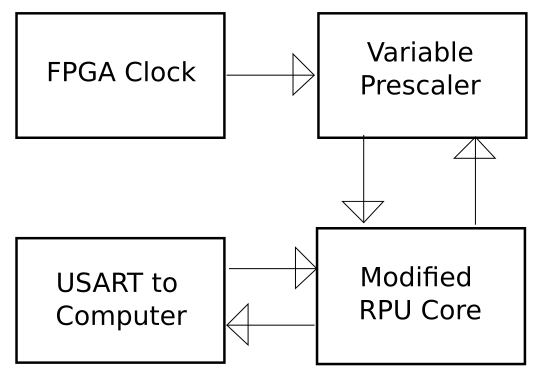
\includegraphics[width=0.5\textwidth]{CompSprint.png}
		\caption{Computation Sprinting Implementation}
		\label{CompSprint}
	\end{figure}
	
	\subsubsection{Sprint Switching}
		A subsection of the computation sprinting design would be to consider a sprint switching design. This methodology considers the tendency of hotspots to build around cores. Implementing hotspot management techniques would be ideal for this project, but this method  mostly relies on switching which core is sprinting at any given point in time, so that the total energy in the system stays consistent and hotspots don't overlap.
	\begin{figure}
		\centering
		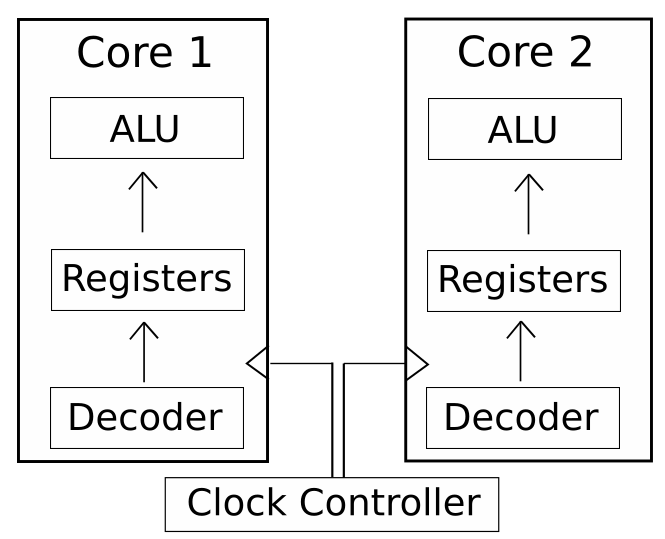
\includegraphics[width=0.5\textwidth]{Switched Sprinting.png}
		\caption{Sprint Switching Implementation}
		\label{Sprint Switching Implementation}
	\end{figure}
	
	\subsubsection{Single Threading Switching}
		A single threaded variant on sprint switching would involve connecting the registers of multiple cores so a core can be sprinted,and when that core becomes too hot, the register values are pushed over to another core, which is then sprinted. The precise method of joining cores would need to be designed to reduce interconnect size. 
	\begin{figure}
		\centering
		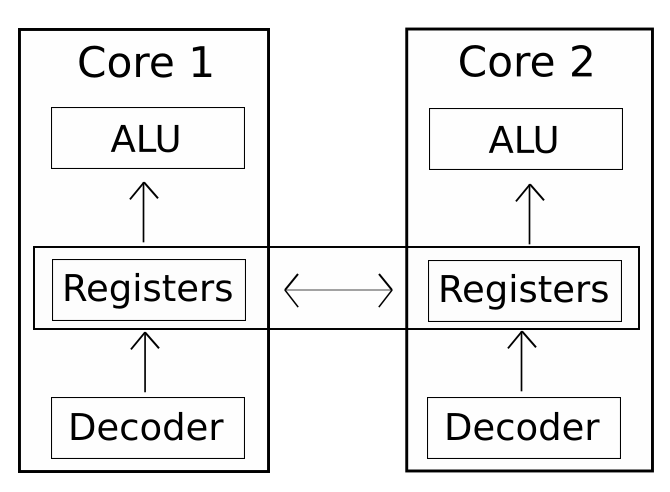
\includegraphics[width=0.5\textwidth]{SingleSwitching.png}
		\caption{Single Threaded Switching Implementation}
		\label{Single Threaded Switching}
	\end{figure}

	\subsection{Memory Driven Computing}
	The memory driven computing implementation would involve placing memory around and between the different cores, as displayed in Figure~\ref{MemDriven}.
	\begin{figure}
		\centering
		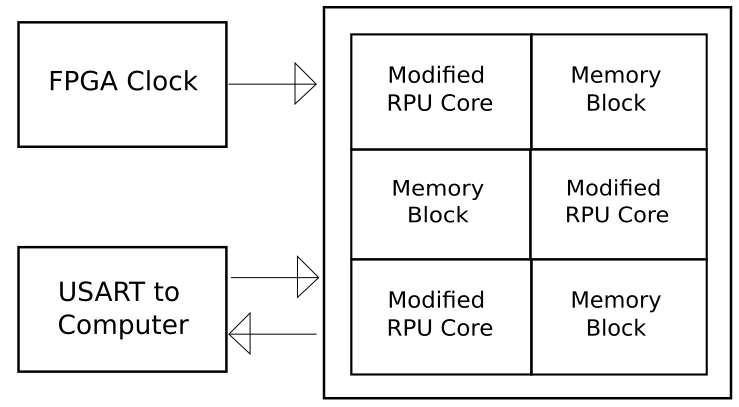
\includegraphics[width=0.5\textwidth]{MemDriven.png}
		\caption{Memory Driven Implementation}
		\label{MemDriven}
	\end{figure}

	\subsection{Heterogeneous Cores}
	The heterogeneous core implementation would involve tying multiple cores together with the main controlling core linking them together as shown in Figure~\ref{HetCores}.
	\begin{figure}
		\centering
		\includegraphics[width=0.5\textwidth]{HetCores.png}
		\caption{Heterogeneous Implementation}
		\label{HetCores}
	\end{figure}

	\subsubsection{Reduced Frequency Cores}
	A variant on the heterogeneous core design methodology would be to use cores that vary by their critical path length. Reducing the maximum clocking frequency of a core reduces the maximum critical path. Using smaller transistors, and taking advantage of the increase area budgets of dark silicon chips, an increased critical path could allow the number of pipelining stages to be reduced. If this can be done in a way that doesn't sacrifice performance, this could be a valuable way to exploit the loosened area constraints. This can also allow cores to be chosen based on how conducive they are to different levels of pipelining.
	\begin{figure}
		\centering
		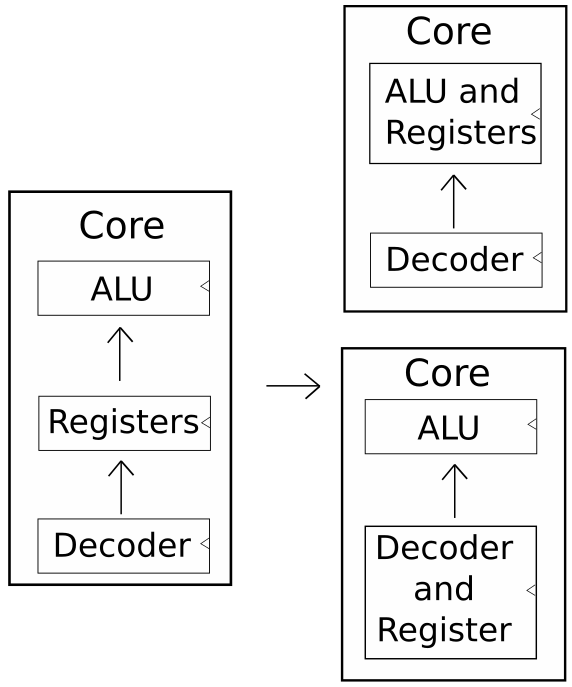
\includegraphics[width=0.5\textwidth]{ReducedFrequencyCores.png}
		\caption{Reduced Frequency Implementation}
		\label{ReducedFreqCores}
	\end{figure}



	
